%!TEX root = <main.tex>
\section{Incremental Inference Optimizations}\label{sec:optimizer}

In this section, we first present the resulting theoretical speedups that can be achieved with incremental inference for popular deep CNN architectures.
We then explain the mechanics of the \textit{incremental inference} operator for a single layer.
Next, we explain how the individual \textit{incremental inference} operator can be used to propagate changes across multiple layers in a deep CNN.
Finally, we explain how we combine \textit{incremental inference} along with \textit{multi-query optimizations} (MQO) to improve the performance of occlusion experiment workload which requires multiple CNN inference requests.

\subsection{Expected Speedups}
We now explain why there is a potential for incremental computation and estimate the upper-bounds for the expected speedups.
In the case of incremental updates only a smaller spatial context having a width $W_{\mathcal{P}:l}$ ($W_{\mathcal{P}:l}<=W_{\mathcal{O}:l}$) and height $H_{\mathcal{P}:l}$ ($H_{\mathcal{P}:l}<=H_{\mathcal{O}:l}$) is needed to be recomputed.
The amount of computations required for the incremental computation $Q_{inc:l}$ and total amount of incremental computations $Q_{inc}$ required for the entire set of convolution layers $L$ will be smaller than the full computation values explained in Section 3, and can be calculated as per Equation ~(\ref{eqn:inc_local}) and ~(\ref{eqn:inc_all}).

\begin{align}
\label{eqn:inc_local}
Q_{inc:l} =&~ (C_{\mathcal{I}:l} \times H_{\mathcal{K}:l} \times W_{\mathcal{K}:l}) \times (C_{\mathcal{O}:l} \times H_{\mathcal{P}:l} \times W_{\mathcal{P}:l})\\
\label{eqn:inc_all}
Q_{inc} =&~ \sum_{l \in L} Q_{inc:l}
\end{align}


Notice that in both full and incremental formulations, computational cost calculation takes into account the dimensions of the output or the output patch.
The output dimensions can be determined using the dimensions of the input and other parameters as explained in Section 3.2.
In Section 4.2 we show that the dimensions of the output patch can also be predetermined using the input patch dimensions.
Using the above quantities we define a new metric named \textit{theoretical speedup} , which is the ratio between the total full computational cost $Q$ and total incremental computation cost $Q_{inc}$ (see Equation ~(\ref{eqn:redundancy_ratio})).
This ratio essentially acts as a surrogate for the theoretical upper-bound for computational and runtime savings that can be achieved by applying incremental computations to Deep CNNs.

\begin{align}
\label{eqn:redundancy_ratio}
\text{theoretical speedup} =&~ \frac{Q}{Q_{inc}}
\end{align}


\begin{figure}[t]
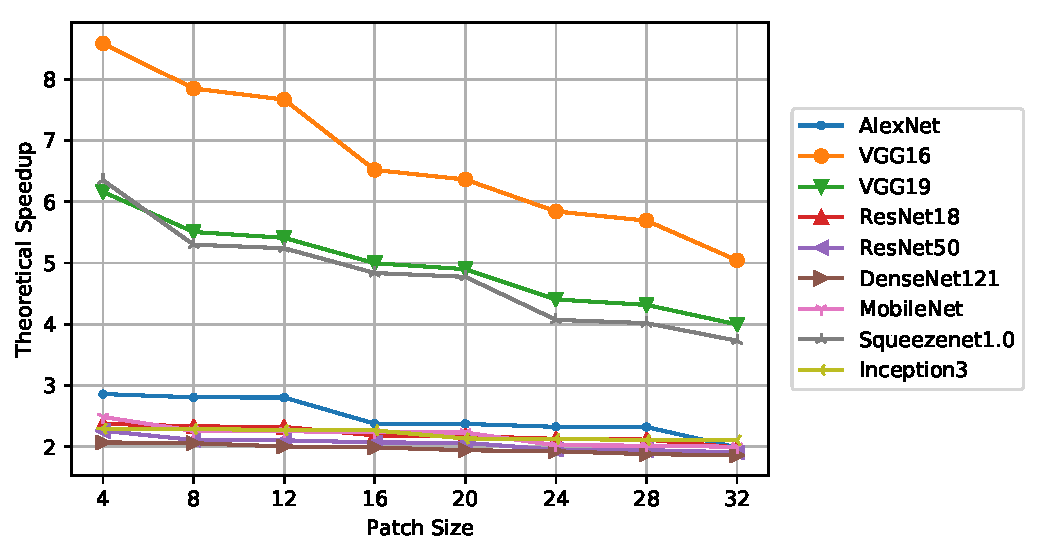
\includegraphics[width=\columnwidth]{images/redundancy_ratio}
\caption{Theoretical speedup for popular CNN architectures with \textit{incremental inference}.}
\label{fig:redundancy_ratio}
\end{figure}

We analyze the theoretical speedup that can be achieved with the \textit{incremental inference} approach when a square occlusion patch is placed on the center\footnote{If the occlusion patch is placed towards a corner of the input image the theoretical speedup will be slightly higher.
But placing the occlusion patch on the center gives us a worst-case estimate.} of the input image.
Figure \ref{fig:redundancy_ratio} shows the results.
VGG16 model results in the maximum theoretical speedup and DenseNet121 model has the lowest theoretical speedup.
Most CNN architectures result in a theoretical speedup between 2-3.
The theoretical speedup for a CNN with \textit{incremental inference} is determined by the characteristics of its architecture such as the number of layers, the sizes of the filter kernels, and the filter stride values.
For example, VGG16 which uses small Convolution filter kernels and strides incurs a very high computational cost (15 GFLOPs) for a single full inference.
However, as the change propagation rate with small filter sizes and strides is small, significant computational savings and runtime speedups can be achieved with incremental inference.
These speedups are significant specially in the human in the loop interactive mode.
For example, with VGG-16 if the original approach would take 1 minute on GPU to execute, it will now take roughly 10 seconds to execute and hence is more amenable for interactive diagnosis of CNN predictions.
On the CPU environment, this implies if a VGG-16 occlusion experiment would take 6 minutes to execute, it will now take only 1 minute to execute and hence will enable significant computational savings and runtime reductions.
Even though for most CNNs the theoretical speedup with incremental inference varies between 2-3, incremental inference approach lays the foundation for the other approximate inference optimizations in \system~ which combined together yields higher speedups.
We next show how to get as close to the above calculated theoretical speedup as possible by combining incremental inference and multi-query optimization.


\subsection{Incremental Inference: Of a Single Layer}\label{sec:inc_computation}
As explained earlier, occlusion experiments in its naive form perform many redundant computations.
In order to avoid these redundancies, layers in a CNN have to be change-aware and operate in an incremental manner, i.e., reuse previous computations as much as possible and compute only the required ones.
In this section, we focus only on transformations that operate at the granularity of a local spatial context (i.e. Convolution and Pooling) as other types either have no redundancies (global context transformations) or are trivial to make change-aware (point transformations) as explained in Section 3.2.

\vspace{2mm}
\noindent \textbf{Calculating the Coordinates and Dimensions of Propagating Patches.} The coordinates and the dimensions (i.e. height and width) of the modified patch in the output tensor of $l^{th}$ layer caused by a modified patch in the input tensor are determined by the coordinates and the dimensions of the input patch, sizes of the filter kernel $H_{\mathcal{K}:l}$ and $W_{\mathcal{K}:l}$, padding values $P_{x:l}$ and $P_{y:l}$, and the strides $S_{x:l}$ and $S_{y:l}$.
For example, consider the simplified demonstration showing a cross-section of input and output in Figure \ref{fig:dimensions}.
We use a coordinate system whose origin is placed at the top left corner of the input.
A patch marked in red is placed on the input starting at $x^\mathcal{I}_{\mathcal{P}:l}, y^\mathcal{I}_{\mathcal{P}:l}$ coordinates and has a height of $H^\mathcal{I}_{\mathcal{P}:l}$ and width of $W^\mathcal{I}_{\mathcal{P}:l}$.
The updated patch in the output starts at $x^\mathcal{O}_{\mathcal{P}:l}, y^\mathcal{O}_{\mathcal{P}:l}$ and has a height of $H^\mathcal{O}_{\mathcal{P}:l}$ and width of $W^\mathcal{O}_{\mathcal{P}:l}$.
Note that due to the overlapping nature of filter positions, to compute the output patch, transformations have to read a slightly larger context than the updated patch.
This ``read-in context'' is shown by the blue shaded area in Figure \ref{fig:dimensions}.
The starting coordinates of this read-in patch are denoted by $x^\mathcal{R}_{\mathcal{P}:l}, y^\mathcal{R}_{\mathcal{P}:l}$ and the dimensions are denoted by $W^\mathcal{R}_{\mathcal{P}:l}, H^\mathcal{R}_{\mathcal{P}:l}$.
Table \ref{table:optimizer_symbols} summarizes these additional notation.
The relationship between the coordinates and dimensions in the horizontal axis (similarly on the vertical axis) can be expressed as follows:

\begin{figure}[t]
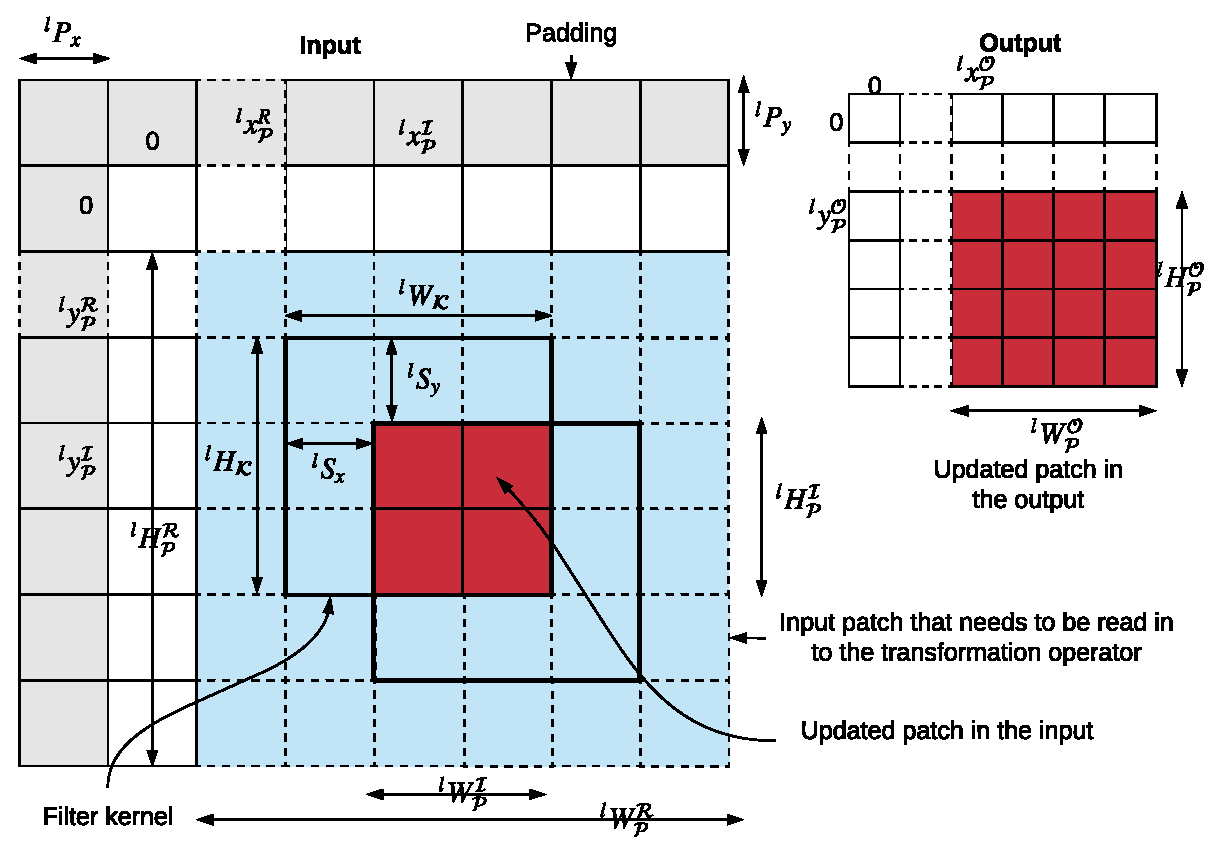
\includegraphics[width=\columnwidth]{images/dimensions}
\caption{Simplified representation of input and output patch coordinates and dimensions of Convolution and Pool transformations.}
\label{fig:dimensions}
\end{figure}

\begin{align}
\label{eqn:xcoordinate}
x^\mathcal{O}_{\mathcal{P}:l} =&~ max\big(\lceil (P_{x:l} + x^\mathcal{I}_{\mathcal{P}:l} - W_{\mathcal{K}:l} + 1)/S_{x:l} \rceil, 0\big)\\
\label{eqn:patchwidth}
W^\mathcal{O}_{\mathcal{P}:l} =&~ min\big(\lceil (W^\mathcal{I}_{\mathcal{P}:l} + W_{\mathcal{K}:l} - 1)/ S_{x:l} \rceil, W_{\mathcal{O}:l}\big)\\
\label{eqn:xreadcoordinate}
x^\mathcal{R}_{\mathcal{P}:l} =&~ x^\mathcal{O}_{\mathcal{P}:l} \times S_{x:l} - P_{x:l}\\
\label{eqn:readpatchwidth}
W^\mathcal{R}_{\mathcal{P}:l} =&~ W_{\mathcal{K}:l} + (W^\mathcal{O}_{\mathcal{P}:l}-1) \times S_{x:l}
\end{align}

% \begin{align}
% \label{eqn:xcoordinate}
% x^\mathcal{O}_\mathcal{P} =&~ max\big(\lceil (P_x + x^\mathcal{I}_\mathcal{P} - W_\mathcal{K} + 1)/S_x \rceil, 0\big)\\
% \label{eqn:ycoordinate}
% y^\mathcal{O}_\mathcal{P} =&~ max\big(\lceil (P_y + y^\mathcal{I}_\mathcal{P} - H_\mathcal{K} + 1)/S_y \rceil, 0\big)
% \end{align}

% \begin{align}
% \label{eqn:patchwidth}
% W^\mathcal{O}_\mathcal{P} =&~ min\big(\lceil (W^\mathcal{I}_\mathcal{P} + W_\mathcal{K} - 1)/S_x \rceil, W_{\mathcal{O}}\big)\\
% \label{eqn:patchheight}
% H^\mathcal{O}_\mathcal{P} =&~ min\big(\lceil (H^\mathcal{I}_\mathcal{P} + H_\mathcal{K} - 1)/S_y \rceil, H_{\mathcal{O}}\big)
% \end{align}

% \begin{align}
% \label{eqn:xreadcoordinate}
% x^\mathcal{R}_\mathcal{P} =&~ x^\mathcal{O}_\mathcal{P} \times S_x - P_x\\
% \label{eqn:yreadcoordinate}
% y^\mathcal{R}_\mathcal{P} =&~ y^\mathcal{O}_\mathcal{P} \times S_y - P_y
% \end{align}

% \begin{align}
% \label{eqn:readpatchwidth}
% W^\mathcal{R}_\mathcal{P} =&~ W_\mathcal{K} + (W^\mathcal{O}_\mathcal{P}-1) \times S_x\\
% \label{eqn:readpatchheight}
% H^\mathcal{R}_\mathcal{P} =&~ H_\mathcal{K} + (H^\mathcal{O}_\mathcal{P}-1) \times S_y
% \end{align}

Equation (\ref{eqn:xcoordinate}) calculates the starting coordinates of the output patch.
Use of padding effectively shifts the coordinate system and therefore $P_{x:l}$ is added to correct it.
Due to the overlapping nature of filter kernels, the affected span of the updated patch in the input will be increased by $W_{\mathcal{K}:l}-1$ amount and hence needs to be subtracted from the input coordinate $x^\mathcal{I}_{\mathcal{P}:l}$ (a filter of size $W_{\mathcal{K}:l}$ that is placed starting at $x^\mathcal{I}_{\mathcal{P}:l} - W_{\mathcal{K}:l} + 1$ will see the new change at $x^\mathcal{I}_{\mathcal{P}:l}$).
Equation (\ref{eqn:patchwidth}) calculates the width of the output patches.
Once the output patch coordinate and width are calculated it is straightforward to calculate the read-in patch coordinate as per Equation (\ref{eqn:xreadcoordinate}) and the width as per Equation (\ref{eqn:readpatchwidth}).


\begin{table}[t]
  \centering
  \caption{Additional symbols used in the Section \ref{sec:optimizer} and Section \ref{sec:approx}}
  \scalebox{0.8}{\begin{tabular}{p{2cm}p{7.5cm}}
    \toprule
    \textbf{Symbol} & \textbf{Meaning}\\
    \midrule \midrule
    $x^\mathcal{I}_{\mathcal{P}:l}, y^\mathcal{I}_{\mathcal{P}:l}$ & Starting coordinates of the input patch for the $l^{th}$ layer\\
    \midrule
    $x^\mathcal{R}_{\mathcal{P}:l}, y^\mathcal{R}_{\mathcal{P}:l}$ & Starting coordinates of the patch that needs to be read in for the $l^{th}$ layer transformation\\
    \midrule
    $x^\mathcal{O}_{\mathcal{P}:l}, y^\mathcal{O}_{\mathcal{P}:l}$ & Starting coordinates of the output patch for the $l^{th}$ layer\\
    \midrule
    $H^\mathcal{I}_{\mathcal{P}:l}, W^\mathcal{I}_{\mathcal{P}:l}$ & Height and width of the input patch for the $l^{th}$ layer\\
   	\midrule
   	$H^\mathcal{R}_{\mathcal{P}:l}, W^\mathcal{R}_{\mathcal{P}:l}$ & Height and width of the patch that needs to be read in for the $l^{th}$ layer transformation\\
   	\midrule
   	$H^\mathcal{O}_{\mathcal{P}:l}, W^\mathcal{O}_{\mathcal{P}:l}$ & Height and width of the output patch for the $l^{th}$ layer\\
    \midrule
    $\tau$ & Projective field threshold\\
    \midrule
    $r_{drill-down}$ & Stage two drill-down fraction used in \textit{adaptive drill-down}\\
    \bottomrule
  \end{tabular}}
\label{table:optimizer_symbols}
\end{table}

\vspace{2mm}
\noindent \textbf{Incremental Inference Operation.} For layer $l$, given the original transformation function $T_{:l}$, pre-materialized input tensor $\mathcal{I}_{:l}$, updated input patch $\mathcal{P}^\mathcal{O}_{:l}$, and the above calculated coordinates and dimensions of the input, output, and read-in patches, the output patch $\mathcal{P}^\mathcal{O}_{:l}$ can be calculated as follows:

\begin{align}
\label{eqn:readin}
\mathcal{U} =&~ \mathcal{I}_{:l}[:,x^\mathcal{R}_{\mathcal{P}:l}:x^\mathcal{R}_{\mathcal{P}:l}+W^\mathcal{R}_{\mathcal{P}:l}, y^\mathcal{R}_{\mathcal{P}:l}: y^\mathcal{R}_{\mathcal{P}:l}+ H^\mathcal{R}_{\mathcal{P}:l}]\\
\label{eqn:superposition}
\mathcal{U} =&~ \mathcal{U} \bm\circ_{(x^\mathcal{I}_{\mathcal{P}:l}-x^\mathcal{R}_{\mathcal{P}:l}),(y^\mathcal{I}_{\mathcal{P}:l}-y^\mathcal{R}_{\mathcal{P}:l})} \mathcal{P}^{\mathcal{I}}_{:l}\\
\label{eqn:callt}
\mathcal{P}^\mathcal{O}_{:l} =&~ T_{:l}(\mathcal{U})
\end{align}

Equation (\ref{eqn:readin}) reads the read-in context $\mathcal{U}$ from the pre-materialized input $\mathcal{I}_{:l}$. Equation (\ref{eqn:superposition}) superimposes the input patch $\mathcal{P}^\mathcal{I}_{:l}$ on it.
Finally, Equation (\ref{eqn:callt}) calculates the modified output patch $\mathcal{P}^{\mathcal{O}}_{:l}$ by invoking $T$ on $\mathcal{U}$.


\subsection{Propagating Patches across Layers}

\vspace{2mm}
\noindent \textbf{CNNs with a Sequence of Layers.} In a CNN composed of a sequence of layers, the updated output patch $\mathcal{P}^{\mathcal{O}}_{:l}$ of layer $l$ is fed as the input to layer $l+1$ along with the pre-materialized input $\mathcal{I}_{:l+1}$ from the original image.
However, at a boundary of a local context transformation and a global context transformation, such as in Convolution $\rightarrow$ Fully-Connected or Pool $\rightarrow$ Fully-Connected, the full updated output has to be materialized instead of propagating only the updated patches.

\vspace{2mm}
\noindent \textbf{Extending to DAG like CNNs.} In most CNNs, especially the newer and popular ones, the layers are organized into the more generic directed acyclic graph (DAG) structure instead of a simple sequence.
In addition to the different CNN layers, theses CNNs contain two linear algebra operators: element-wise addition and depth-wise concatenation which are used to merge two branches in the DAG. 
Element-wise addition operator requires the two input tensor to have exact same dimensions.
Depth-wise concatenation requires them to have the same height and width dimensions.

Consider a situation for these operators as shown in Figure \ref{fig:la_operators} where the first input has an incremental update starting at coordinates $x^\mathcal{I}_{\mathcal{P}_1:l},y^\mathcal{I}_{\mathcal{P}_1:l}$ with dimensions of $H^\mathcal{I}_{\mathcal{P}_1:l}$ and $W^\mathcal{I}_{\mathcal{P}_1:l}$ and for the second input starting at coordinates $x^\mathcal{I}_{\mathcal{P}_2:l},y^\mathcal{I}_{\mathcal{P}_2:l}$ with dimensions of $H^\mathcal{I}_{\mathcal{P}_2:l}$ and $W^\mathcal{I}_{\mathcal{P}_2:l}$.
In this case, the coordinates and dimensions of both output and read-in contexts will be the same, computing them essentially requires finding the bounding box of the two input patches.
For the horizontal axis (similarly for the vertical axis) this can be expressed as follows:

\begin{figure}[t]
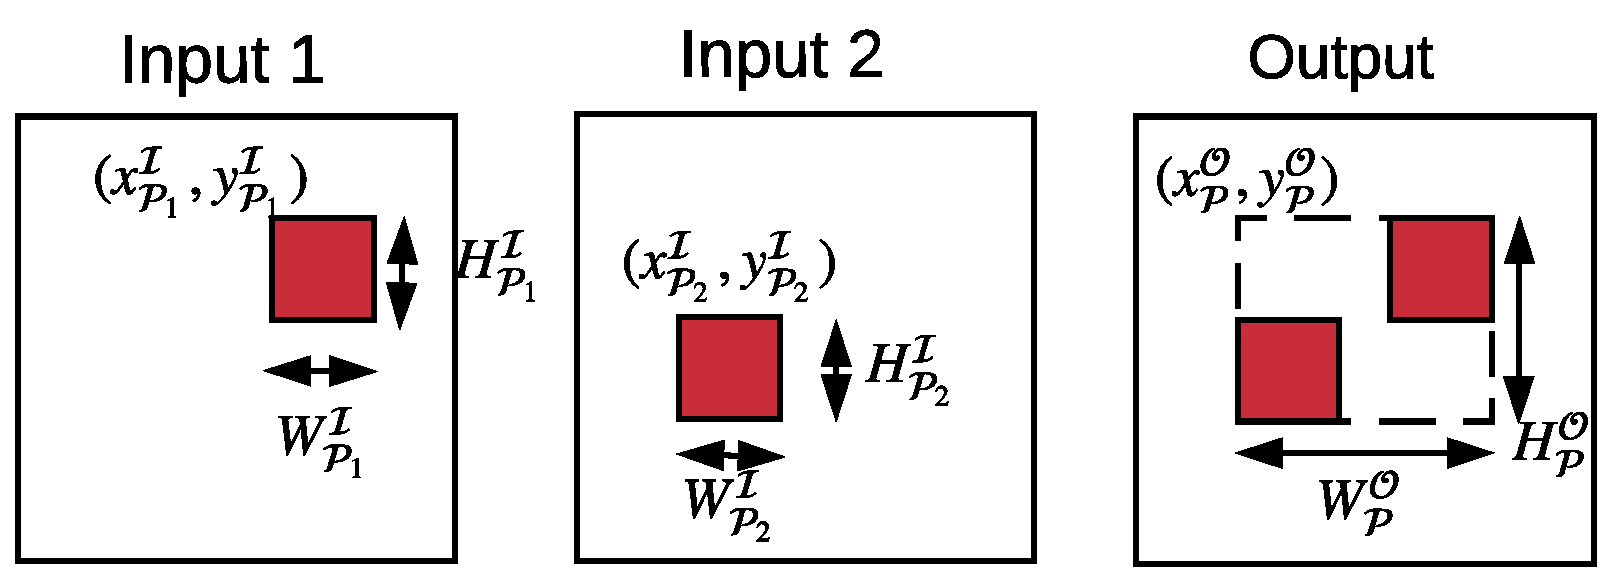
\includegraphics[width=\columnwidth]{images/la_operators}
\caption{Input-output coordinate and dimension mapping for element-wise addition and depth-wise concatenation.}
\label{fig:la_operators}
\end{figure}

\begin{align}
\begin{split}
x^\mathcal{O}_{P:l} =&~ \texttt{min}(x^\mathcal{I}_{\mathcal{P}_1:l}, x^\mathcal{I}_{\mathcal{P}_2:l})\\
% y^\mathcal{O}_\mathcal{P} = y^\mathcal{R}_\mathcal{P} =&~ \texttt{min}(y^\mathcal{I}_{\mathcal{P}_1},y^\mathcal{I}_{\mathcal{P}_2})\\
% \label{eqn:lapatchwidth}
W^\mathcal{O}_{\mathcal{P}:l} =&~ \texttt{max}(x^\mathcal{I}_{\mathcal{P}_1:l}+W^\mathcal{I}_{\mathcal{P}_1:l},x^\mathcal{I}_{\mathcal{P}_2:l}+W^\mathcal{I}_{\mathcal{P}_2:l}) -\texttt{min}(x^\mathcal{I}_{\mathcal{P}_1:l},x^\mathcal{I}_{\mathcal{P}_2:l})
% H^\mathcal{O}_\mathcal{P} = H^\mathcal{R}_\mathcal{P} =&~ \texttt{max}(y^\mathcal{I}_{\mathcal{P}_1}+H^\mathcal{I}_{\mathcal{P}_1},y^\mathcal{I}_{\mathcal{P}_2}+H^\mathcal{I}_{\mathcal{P}_2})-\texttt{min}(y^\mathcal{I}_{\mathcal{P}_1},y^\mathcal{I}_{\mathcal{P}_2})
\end{split}
\end{align}

\subsection{Multi-Query Inference}
As explained in Section \ref{sec:problem}, occlusion experiments require performing multiple CNN inferences with each corresponding to a specific occlusion patch position.
Each of these individual inference request is analogous to a \textit{query} in the RDBMs context.
Coupled with \textit{incremental inference} optimization, these multiple inference requests provide opportunities to apply \textit{multi-query optimization} style optimization to the occlusion experiment workload.
We materialize all intermediate tensors in the CNN once for the unmodified image and reuse it for all remaining queries with incremental computations.
To the best of our knowledge, this is the first instance of applying incremental view maintenance combined with multi-query optimization to improve performance in a data system.
We also apply system specific optimizations to improve performance in the high throughput GPU environment.

\vspace{2mm}
\noindent \textbf{Batched Incremental Inference.} In \system~ \textit{incremental inference} optimization is applied on top of the currently dominant approach of performing CNN inference on batches of images, with batch size selected to optimize hardware utilization.
Each image in the batch corresponds to an occluded instance of the original image.
Batched inference is important as it reduces the per-image inference time by amortizing the fixed overheads.
In our experiments we found that this simple optimization alone can give up to ~1.4X speedups in the CPU environment and ~2X speedups on the GPU environment compared to the per-image inference approach.
Algorithm \ref{alg:incinference} presents the \textit{batched incremental inference} operator for the $l^{th}$ layer formally.

\begin{algorithm}
    \caption{Batched Incremental Inference Algorithm}
    \label{alg:incinference}
    \begin{flushleft}
     \hspace*{1mm} \textbf{Input:} \\
     \hspace*{3mm} $T_{:l}$ : \textit{Original Transformation function}\\
     \hspace*{3mm} $\mathcal{I}_{:l}$ : \textit{Pre-materialized input from original image}\\
     \hspace*{3mm} $[\mathcal{P^I}_{1:l},...,\mathcal{P^I}_{n:l}]$ : \textit{Input patches}\\
     \hspace*{3mm} $[(x^\mathcal{I}_{\mathcal{P}_1:l},y^\mathcal{I}_{\mathcal{P}_1:l}),...,(x^\mathcal{I}_{\mathcal{P}_n:l},y^\mathcal{I}_{\mathcal{P}_n:l})]$ : \textit{Input patch coordinates}\\
     \hspace*{3mm} $W^\mathcal{I}_{\mathcal{P}:l},H^\mathcal{I}_{\mathcal{P}:l}$ : \textit{Input patch dimensions}
    \end{flushleft}

    \begin{flushleft}
     \hspace*{1mm} \textbf{Output:}\\
     \hspace*{3mm} $[\mathcal{P^O}_{1:l},...,\mathcal{P^O}_{n:l}]$ : \textit{Output patches}\\
     \hspace*{3mm} $[(x^\mathcal{O}_{\mathcal{P}_1:l},y^\mathcal{O}_{\mathcal{P}_1:l}),...,(x^\mathcal{O}_{\mathcal{P}_n:l},y^\mathcal{O}_{\mathcal{P}_n:l})]$ : \textit{Output patch coordinates}\\
     \hspace*{3mm} $W^\mathcal{O}_{\mathcal{P}:l},H^\mathcal{O}_{\mathcal{P}:l}$ : \textit{Output patch dimensions}
    \end{flushleft}

    \begin{algorithmic}[1]
    \Procedure{BatchedIncrementalInference}{}
    \State \textit{Calculate} $[(x^\mathcal{O}_{\mathcal{P}_1:l},y^\mathcal{O}_{\mathcal{P}_1:l}),...,(x^\mathcal{O}_{\mathcal{P}_n:l},y^\mathcal{O}_{\mathcal{P}_n:l})]$ 
    \State \textit{Calculate} ($W^\mathcal{O}_{\mathcal{P}:1},H^\mathcal{O}_{\mathcal{P}:l}$)
    \State \textit{Calculate} $[(x^\mathcal{R}_{\mathcal{P}_1:l},y^\mathcal{R}_{\mathcal{P}_1:l}),...,(x^\mathcal{R}_{\mathcal{P}_n:l},y^\mathcal{R}_{\mathcal{P}_n}:l)]$
    \State \textit{Calculate} ($W^\mathcal{R}_{\mathcal{P}:l},H^\mathcal{R}_{\mathcal{P}:l}$)
    \State \textit{Initialize} $\mathcal{U} \in \mathcal{\rm I\!R}^{n \times \texttt{depth}(\mathcal{I}_{:l}) \times H^\mathcal{R}_{\mathcal{P}:l} \times W^\mathcal{R}_{\mathcal{P}:l}}$

    \For{\texttt{i in [1,...,n]}}\label{alg:line:memcpy_loop}
        \State $T_1 \gets \mathcal{I}_{:l}[:,x^\mathcal{R}_{\mathcal{P}_i:l}:x^\mathcal{R}_{\mathcal{P}_i:l}+W^\mathcal{R}_{\mathcal{P}:l},y^\mathcal{R}_{\mathcal{P}_i:l}:y^\mathcal{R}_{\mathcal{P}_i:l}+H^\mathcal{R}_{\mathcal{P}:l}]$ 
        \State $T_2 \gets T_1 \bm\circ_{(x^\mathcal{I}_{\mathcal{P}_i:l}-x^\mathcal{R}_{\mathcal{P}_i:l}),(y^\mathcal{I}_{\mathcal{P}_i:l}-y^\mathcal{R}_{\mathcal{P}_i:l})} \mathcal{P}_{i:l}$
        \State $\mathcal{U}[i,:,:] \gets T_2$
    \EndFor

    \State $[\mathcal{P}^\mathcal{O}_{1:l},...,\mathcal{P}^\mathcal{O}_{n:l}] \gets T(\mathcal{U})$ \Comment{Batched version}
    \State \textbf{return} $[\mathcal{P}^\mathcal{O}_{1:l},...,\mathcal{P}^\mathcal{O}_{n:l}]$,
    \State \hspace*{5mm} $[(x^\mathcal{O}_{\mathcal{P}_1:l},y^\mathcal{O}_{\mathcal{P}_1:l}),...,(x^\mathcal{O}_{\mathcal{P}_n:l},y^\mathcal{O}_{\mathcal{P}_n:l})],$ ($W^\mathcal{O}_{\mathcal{P}:l},H^\mathcal{O}_{\mathcal{P}:l}$) 
    \EndProcedure
    \end{algorithmic}

% \eat{%Maybe in the Appendix
%     \vspace*{-2mm}
%     \hrulefill
    
%     \begin{flushleft}
%      \hspace*{4mm} \textbf{Input:}\\
%      \hspace*{8mm} $\mathcal{O}$ : \textit{Pre-materialized output from original image}\\
%      \hspace*{8mm} $[\mathcal{P}^\mathcal{O}_1,...,\mathcal{P}^\mathcal{O}_n]$ : \textit{Output patches}\\
%      \hspace*{8mm} $[(x^\mathcal{O}_{\mathcal{P}_1},y^\mathcal{O}_{\mathcal{P}_1}),...,(x^\mathcal{O}_{\mathcal{P}_n},y^\mathcal{O}_{\mathcal{P}_n})]$ : \textit{Output patch coordinates}\\
%     \end{flushleft}

%     \begin{flushleft}
%      \hspace*{4mm} \textbf{Output:}\\
%      \hspace*{8mm} $O\textrm'$ : \textit{Updated output}
%     \end{flushleft}
%   \begin{algorithmic}[1]
%     \Procedure{IncrementalToFullProjection}{}
%     \State \textit{Initialize} $\mathcal{O}\textrm' \in \mathcal{\rm I\!R}^{n \times \texttt{depth}(\mathcal{O}) \times \texttt{height}(\mathcal{O}) \times \texttt{width}(\mathcal{O})}$
%     \For{\texttt{i in [1,...,n]}}
%       \State $T \gets \texttt{copy}(O)$
%       \State $\mathcal{O}\textrm'[i,:,:] \gets T \bm\circ_{x^\mathcal{O}_{\mathcal{P}_i},y^\mathcal{O}_{\mathcal{P}_i}} \mathcal{P}^\mathcal{O}_i$
%     \EndFor
%     \State \textbf{return} $\mathcal{O}\textrm'$
%     \EndProcedure
%     \end{algorithmic}
% }
\end{algorithm}


\eat{
The \textproc{BatchedIncrementalInference} procedure takes in the original transformation of the layer, pre-materialized input for the layer corresponding to the original image, a batch of updated patches which are 3D volumes of activation values and their geometric properties as input.
}
Notice that for the first layer, all the elements in the batch of updated patches will be identical as the same occlusion patch (in RGB format) is used.
However, at latter layers they will be different as each input patch will subject to different computations due to different read-in contexts across patches.
First, \textproc{BatchedIncrementalInference} calculates the geometric properties of the output and the read-in contexts.
A temporary input tensor $U$ is initialized to hold the input patches with their read-in contexts.
The \texttt{for} loop iteratively populates $U$ with corresponding patches.
Finally, $T_{:l}$ is applied to $U$ to compute the output patches.
\eat{
It should be noted that pre-materialized input $\mathcal{I}_{:l}$ for the unmodified input image can be reused across multiple batches corresponding the the same image.
}

\vspace{2mm}
\noindent \textbf{GPU Optimized Implementation.}
Through our experiments, we found that even though a straight-forward implementation of \textit{batched incremental inference} approach as shown in Algorithm \ref{alg:incinference} produces expected speedups for the CPU environment, it performs poorly on the GPU environment.
The \texttt{for} loop on the line \ref{alg:line:memcpy_loop} of Algorithm \ref{alg:incinference} is essentially preparing the input for $T_{:l}$ by copying values from one part of the memory to another sequentially.
However, in the \textit{multi-query} setting this sequential operation becomes a bottleneck for the GPU implementation, since it cannot exploit the available parallelism of the GPU efficiently.
To overcome this we have extended PyTorch by adding a custom kernel written in CUDA language which performs the input preparation more efficiently by parallelly copying the memory regions for all items in the batch and then invoke the CNN transformation function $T_{:l}$.
More details on the custom GPU kernel implementation is explained in Appendix.
The original transformation function $T_{:l}$, which is provided as an input to the Algorithm \ref{alg:incinference} is already optimized to use the GPU efficiently for a batch of inputs when performing inference.
\red{TODO: Refer to hardware works, e.g. Li Tseng, Lin, Swanson, Yannis on hardware accelerators}


\subsection{Putting it all together}

The high-level steps taken by the end-to-end incremental inference approach for the occlusion experiment can be summarized as follows:

\begin{enumerate}
	\item Take in CNN $f$, image $\mathcal{I}_{:img}$, predicted class label $L$, occlusion patch $\mathcal{P}$, stride $S_{\mathcal{P}}$ for the $\mathcal{P}$, and the set of occluding patch placement positions $G$ as input.
	\item Pre-materialize output of all the transformations in $f$ by feeding in $\mathcal{I}_{:img}$.
	%\item Calculate all possible $\mathcal{P}$ positions on $\mathcal{I}_{img}$.
	\item Prepare the occluded images ($\mathcal{I}^{'}_{x,y:img}$ s) corresponding to all positions in $G$.
	\item For batches of $\mathcal{I}^{'}_{x,y:img}$ as the input, invoke the transformations in $f$ in topological order and calculate the corresponding values of heat map $M$.
	\begin{itemize}
		\item For local-context transformation, invoke \textproc{BatchedIncrementalInference}.
		\item For local-context transformation, that feeds in a global context transformation additionally materialize the full updated output.
		\item For all others, invoke the original transformation function.
	\end{itemize}
	\item Return M as the final output.
\end{enumerate}


\section{Approximate Inference Optimizations}\label{sec:approx}
In this Section, we explain \textit{projective field thresholding} and \textit{adaptive drill-down}, which are two \textit{approximate inference} optimizations used in ~\system.
We also explain how \system~ tunes its internal system configuration parameters for these \textit{approximate inference} optimizations.


\subsection{Projective Field Thresholding}
Projective field \cite{le2017receptive, basiccnnoperations} of a CNN neuron is the local region (including the depth) of the output 3-D tensor which is connected to it.
The term is borrowed from the Neuroscience field where it is used to describe the spatiotemporal effects exerted by a retinal cell on all of the outputs of the neuronal circuitry \cite{de2011projective}.
For our work, the notion of projective field is useful as it determines the change propagation path for incremental changes.
The three types of CNN transformations affect the size of the projective field differently.
Point transformations do not change the projective field size while global context transformations increase it to the maximum.
Transformations that operate on a local spatial context increase it gradually.
The amount of increase in a local context transformation is determined by the filter size and stride parameters.
At every transformation, the size of the projective field will increase linearly by the filter size and multiplicatively by the stride value.

\begin{figure}[t]
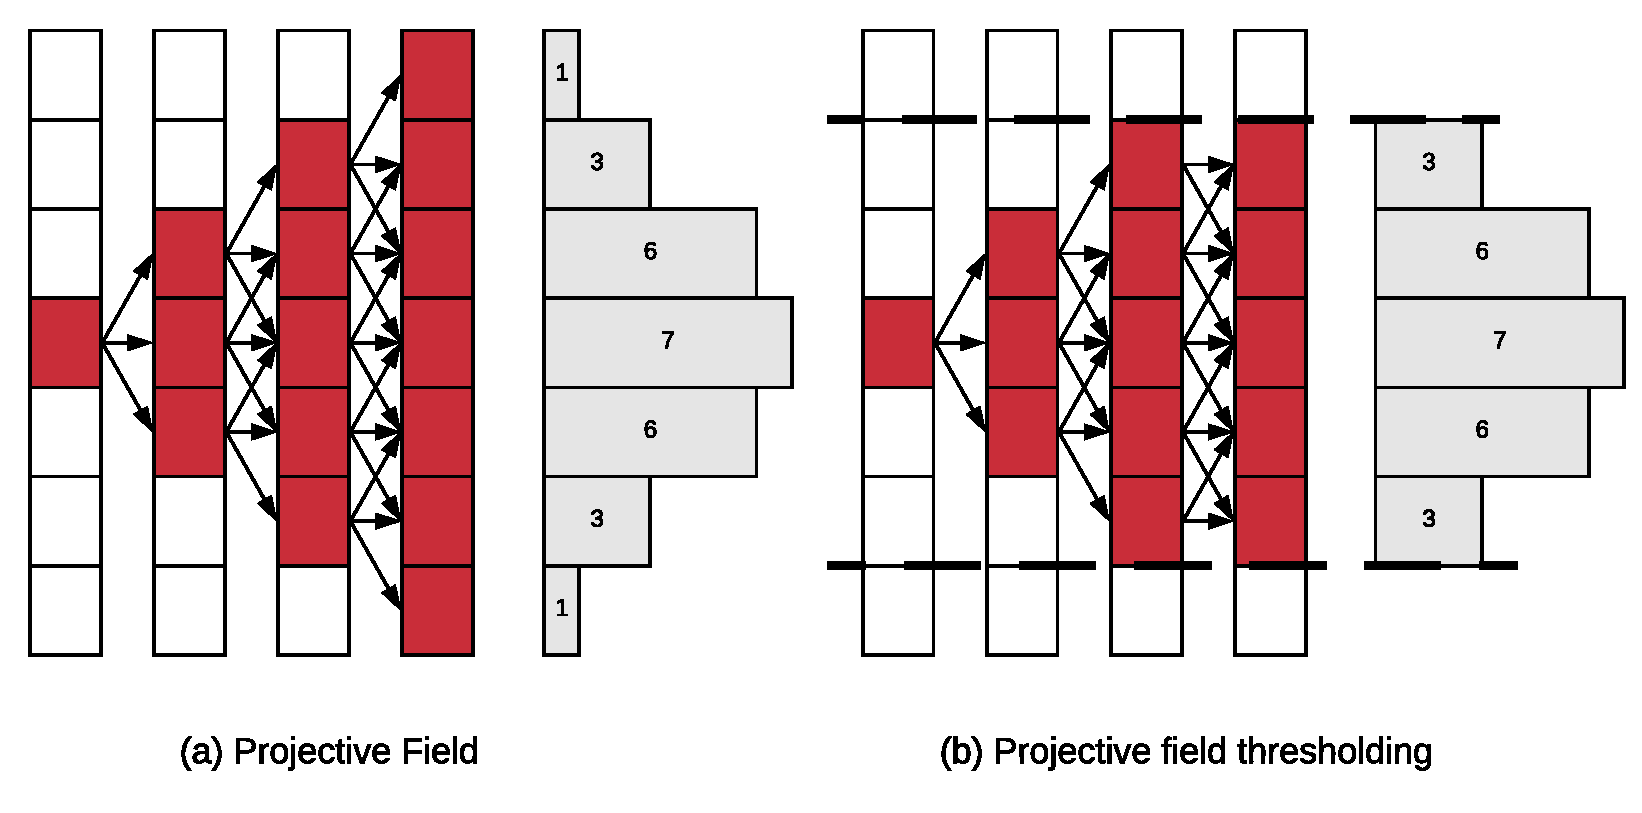
\includegraphics[width=\columnwidth]{images/pf_truncate}
\caption{(a) One dimensional Convolution demonstrating projective field growth (filter size = 2, stride = 1). (b) \textit{Projective field thresholding} with $\tau = 5/7$.}
\label{fig:pf_truncate}
\end{figure}

Because of the projective field growth, even though there will be many computational redundancies in the early layers, towards the latter layers it will decrease or even have no redundancies.
However, we empirically found that the projective field growth can be restrained up to a certain extent without significantly sacrificing the accuracy.
For a more intuitive understanding of why this would work consider the simplified 1-D Convolution example shown in Figure \ref{fig:pf_truncate} (a).
In the example, a single neuron is modified (marked in red) and a filter of size three is applied with a stride of one repeatedly four times.
Since the filter size is three, each updated neuron will propagate the change to three neurons in the next output layer causing the projective field to grow linearly.
The histogram at the end of the fourth layer shows the number of unique paths that are available between each output neuron and the originally updated neuron in the first layer.
It can be seen that this distribution resembles a Gaussian where many of the paths are connected to the central region.
The amount of change in the output layer is determined by both the number of unique paths and also the individual weights of the connections.
It can be shown that the distribution of change in the output layer will converge to a Gaussian distribution provided certain conditions are met for the weight values of the filter kernel (more details in Appendix X).
\eat{
For more details we refer the reader to \cite{luo2016understanding}, where a similar theoretical result has been proved for the receptive field\footnote{Receptive field of a CNN neuron is the local region (including the depth) of the input volume which is connected to it.} of a Deep CNN.
}

As most of the change will be concentrated on the center we introduce the notion of a projective field threshold $\tau ~ (0 < \tau \leq 1)$ which will be used to restrict the growth of the projective field.
It determines the maximum size of the projective field as a fraction of the size of the output.
Figure \ref{fig:pf_truncate} (b) demonstrates the application of projective field thresholding with a $\tau$ value of $5/7$.
From the histogram generated for the projective field thresholding approach, we can expect that much of the final output change is maintained by this approach.

In \system, \textit{projective field thresholding} is implemented on top of \textit{incremental inference} approach by applying set of additional constraints on input-output coordinate mappings. For the horizontal dimension (similarly for vertical dimension) the new set of calculations can be expressed as follows:

\begin{align}
\label{eqn:normal_width_calc}
W^\mathcal{O}_{\mathcal{P}:l} = &~ \texttt{min}\big(\lceil (W^\mathcal{I}_{\mathcal{P}:l} + W_{\mathcal{K}:l} - 1)/S_{x:l} \rceil, W^\mathcal{O}_{\mathcal{P}:l}\big)\\
\label{eqn:check_tau}
\text{If}~ W_{\mathcal{P}:l}^\mathcal{O} & > \texttt{round}(\tau \times W^\mathcal{O}_{:l}):\\
\label{eqn:new_width_calc_with_tau}
& W^\mathcal{O}_{\mathcal{P}:l} = \texttt{round}(\tau \times W^\mathcal{O}_{:l})\\
\label{eqn:new_in_width}
& W^\mathcal{I}_{\mathcal{P}_{new}:l} = W^\mathcal{O}_{\mathcal{P}:l} \times S_{x:l} - W_{\mathcal{K}:l} + 1\\
\label{eqn:new_x_coord}
& x^{\mathcal{I}}_{\mathcal{P}:l} \mathrel{+}= (W^\mathcal{I}_{\mathcal{P}:l} - W^\mathcal{I}_{\mathcal{P}_{new}:l})/2\\
\label{eqn:new_input_width}
& W^\mathcal{I}_{\mathcal{P}:l} = W^\mathcal{I}_{\mathcal{P}_{new}:l}\\
\label{eqn:new_output_x}
x^\mathcal{O}_{\mathcal{P}:l} = & \texttt{max}\big(\lceil (P_{x:l} + x^\mathcal{I}_{\mathcal{P}:l} - W_{\mathcal{K}:l} + 1)/S_{x:l} \rceil, 0\big)
\end{align}

Equation (\ref{eqn:normal_width_calc}) calculates output width assuming no thresholding.
But if the output width exceeds the threshold defined by $\tau$, output width is set to the threshold value as per Equation (\ref{eqn:new_width_calc_with_tau}).
Equation \ref{eqn:new_in_width} calculates the input width that would produce an output of width $W^\mathcal{O}_{\mathcal{P}:l}$ (think of this as making $W^{\mathcal{I}}_{\mathcal{P}:l}$ the subject of equation \ref{eqn:normal_width_calc}).
If the new input width is smaller than the original input width, the starting x coordinate should be updated as per Equation (\ref{eqn:new_x_coord}) such that the updated coordinates correspond to a center crop from the original.
Equation (\ref{eqn:new_input_width}) set the input width to the newly calculated input width and Equation (\ref{eqn:new_output_x}) calculates the x coordinate of the output patch from the updated values.

\begin{figure}[t]
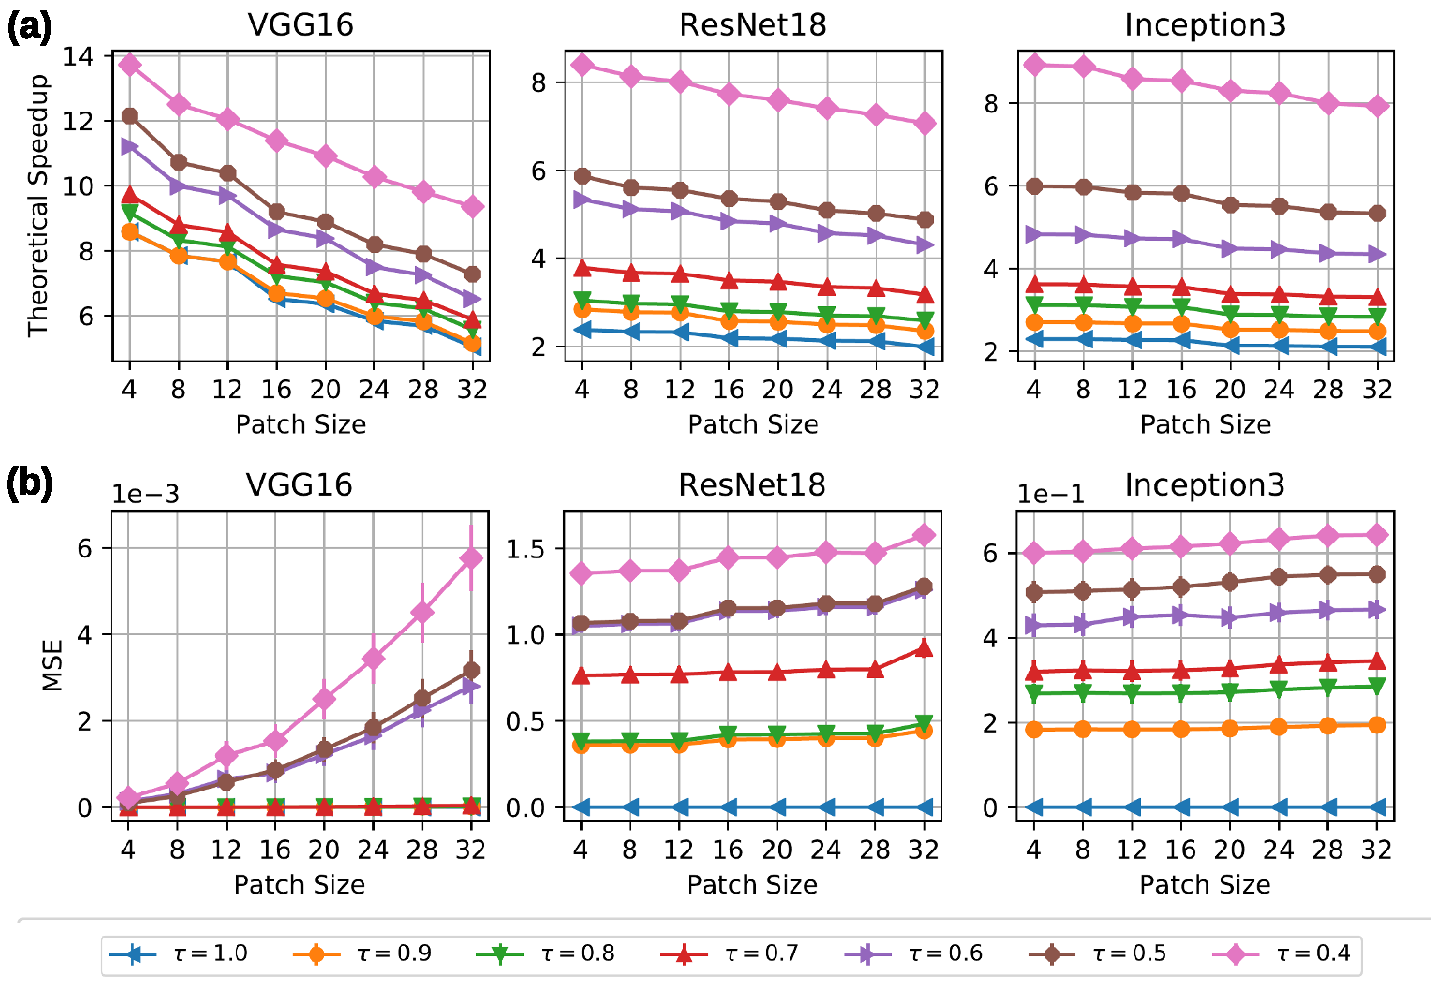
\includegraphics[width=\columnwidth]{images/proj_thresholding}
\caption{(a) Theoretical speedup ratio with projective field thresholding. (b) Mean Square Error between exact and approximate output of the final Convolution or Pool transformation.}
\label{fig:proj_thresholding}
\end{figure}

\vspace{2mm}
\noindent \textbf{Theoretical Speedup with Projective Field Thresholding.}
We analyze the theoretical speedup that can be achieved with \textit{projective field thresholding} approach when a square occlusion patch is placed on the center of the input image.
Figure \ref{fig:proj_thresholding} (a) presents the results.
It can be seen that with increasing $\tau$ attainable theoretical speedup also increases.
We also analyze the mean square error (MSE) between the exact and approximate output tensors produced by the final Convolution or Pool transformation with a black occlusion patch placed on the center of the input image.
The results are shown in Figure \ref{fig:proj_thresholding} (b).
With increasing $\tau$ and increasing patch size we see that the MSE is also increasing.


\subsection{Adaptive Drill-Down}\label{sec:ada-drill-down}
\textit{Adaptive drill-down} approach, which is only applicable in the non-interactive mode, is based on the observation that in many occlusion based explainability workloads, such as in medical imaging, the regions of interest will occupy only a small fraction of the entire image.
In such cases, it is unnecessary to inspect the entire image at a higher resolution with a small stride value for the occlusion patch.
In \textit{adaptive-drill-down} the final occlusion heat map will be generated using a two-stage process.
At the first stage, a low-resolution heat map will be generated by using a larger stride which we call stage one stride $S_1$.
From the heat map generated at stage one, a predefined drill-down fraction $r_{drill-down}$ of regions with highest probability drop for the predicted class is identified.
At stage two a high-resolution occlusion map is generated using the original user provided stride value, also called stage two stride $S_2$, only for the selected region.
A schematic representation of \textit{adaptive drill-down} is shown in Figure \ref{fig:adaptive_drill_down} (a).

% \begin{figure}[t]
% 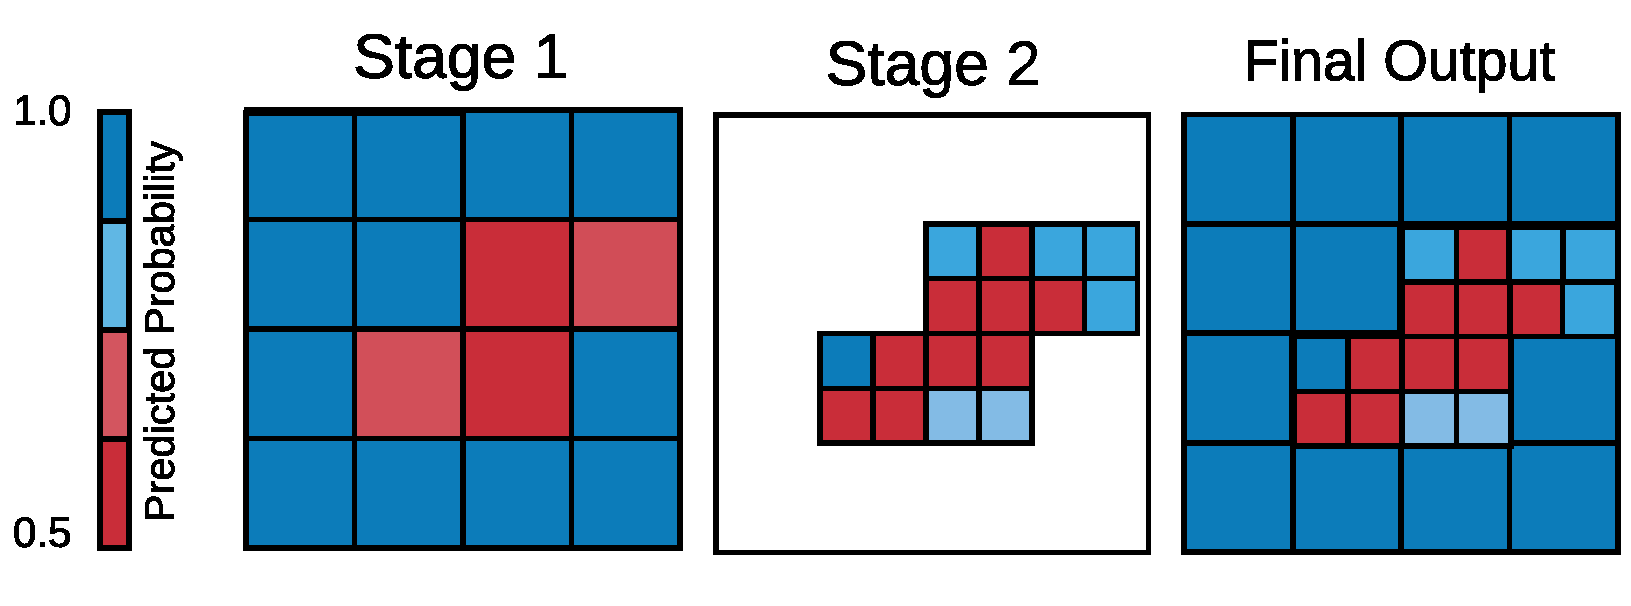
\includegraphics[width=\columnwidth]{images/adaptive-drill-down}
% \caption{Schematic representation of \textit{adaptive drill-down}}
% \label{fig:adaptive-drill-down}
% \end{figure}

The amount of speedup that can be obtained from \textit{adaptive drill-down} is determined by both $r_{drill-down}$ and $S_1$.
If the $r_{drill-down}$ is low, only a small region will have to be examined at a higher resolution and thus it will be faster.
However, this smaller region may not be sufficient to cover all the interesting regions on the image and hence can result in losing important information.
Larger $S_1$ also reduces the overall runtime as it reduces the time taken for stage one.
But it has the risk of misidentifying interesting regions especially when the granularity of those regions are smaller than the occlusion patch size.
The speedup obtained by \textit{adaptive drill-down} approach is equal to the ratio between the number of individual occlusion patch positions generated for the normal and \textit{adaptive drill-down} approaches.
Number of individual occlusion patch positions generated with a stride value of $S$ is proportional to $1/S^2$ (total number of patch positions is equal to $\frac{H_{\mathcal{I}_{img}}}{S} \times \frac{W_{\mathcal{I}_{img}}}{S}$).
Hence the speedup can  be expressed as per Equation \ref{eqn:adaptive-drill-down-eqn}.
Figure \ref{fig:adaptive_drill_down} (b) conceptually shows how the speedup would vary with $S_1$ when $r_{drill-down}$ is fixed and vice versa.

\begin{align}
\label{eqn:adaptive-drill-down-eqn}
\texttt{speedup} = \frac{S^2_1}{S^2_2+r_{drill-down} \times S^2_1}
\end{align}

\begin{figure}[t]
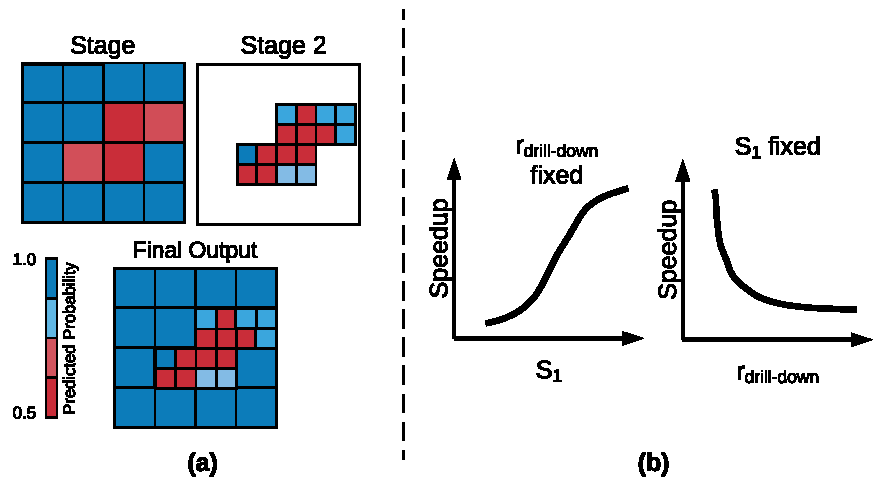
\includegraphics[width=\columnwidth]{images/adaptive_drill_down}
\caption{(a) Schematic representation of \textit{adaptive drill-down}. (b) Conceptual diagram showing the effect of $S_1$ and $r_{drill-down}$ on speedup. }
\label{fig:adaptive_drill_down}
\end{figure}

\subsection{System Tuning}
In this section we explain how \system~ sets its internal configuration parameters for \textit{approximate inference} optimizations.

\vspace{2mm}
\noindent \textbf{Tuning projective field threshold.}
The inaccuracies incurred when applying \textit{projective field thresholding} can cause quality degradation in the generate approximate heat map all the way from indistinguishable changes major structural changes.
To measure this quality degradation we use Structural Similarity (SSIM) Index~\cite{wang2004image}, which is one of the widely used approaches to measure the \textit{human perceived difference} between two similar images.
When applying SSIM index, we treat the original heat map as the reference image with no distortions and the perceived image similarity of the approximate heat map is calculated with reference to it.
The generated SSIM index is a value between $-1$ and $1$, where $1$ corresponds to perfect similarity.
Typically SSIM index values in the range of $0.90-0.95$ are used in practical applications such as image compression and video encoding as at the human perception level they produce indistinguishable distortions.
% For more details on SSIM Index method, we refer the reader to the original SSIM Index paper~\cite{wang2004image}.

Tuning \textit{projective field threshold} $\tau$ is done during a special initial tuning phase.
During this tuning phase \system~ takes in a sample of images (default 30) from the operational workload and evaluates SSIM value of the approximate heat map (compared to the exact heat map) for different $\tau$ values (default values are 1.0, 0.9, 0.8, ..., 0.4).
These $\tau$ versus SSIM data points are then used to fit a second-degree curve.
At the operational time, \system~ requires the user to provide the expected level of quality for the heat maps in terms of a SSIM value.
$\tau$ is then selected from the curve fit to match this target SSIM value.
Figure \ref{fig:system_tuning} (a) shows the SSIM variation and degree two curve fit for different $\tau$ values and three different CNN models for a tuning set (n=30) from OCT dataset.
From the plots, it can be seen that the distribution of SSIM versus $\tau$ lies in a lower dimensional manifold and with increasing $\tau$ SSIM also increases.
Figure \ref{fig:system_tuning} (b) shows the cumulative percentage plots for SSIM deviation for the tune and test sets (n=30) when the system is tuned for a target SSIM of 0.9.
For a target SSIM of 0.9 system picks $\tau$ values of 0.5, 0.7, and 0.9 for VGG16, ResNet18, and Inception3 models respectively.
It can be seen that approximately more than $50\%$ of test cases will result in an SSIM value of 0.9 or greater.
Even in cases where it performs worse than 0.9 SSIM, significant ($95\%-100\%$) portion of them are within +0.1 deviation.

\vspace{2mm}
\noindent \textbf{Tuning adaptive drill-down.}
As explained in section \ref{sec:ada-drill-down} the speedup obtained by \textit{adaptive drill-down} approach is determined by two factors; stage one stride value $S_1$ and drill-down fraction $r_{drill-down}$.
% Figure \ref{fig:adaptive_ssim} shows how the SSIM value of approximate heat maps would change when changing $r_{drill-down}$ and $S_1$ with all other configurations kept fixed.
% A general trend of increasing SSIM with increasing $r_{drill-down}$ and decreasing $S_1$ can be observed from the plots.
For configuring \textit{adaptive drill-down} \system~ requires the user to provide $r_{drill-down}$ and a target \texttt{speedup} value.
$r_{drill-down}$ should be selected based on the user's experience and understanding on the relative size of interesting regions compared to the full image.
This is a fair assumption and in most cases such as in medical imaging, users will have a fairly good understanding on the relative size of the interesting regions.
However, if the user is unable to provide this value \system~ will use a default value of 0.25 as $r_{drill-down}$.
The \texttt{speedup} value basically captures user's input on how much faster the occlusion experiment should run.
Higher speedup values will sacrifice the quality of non-interesting (1-$r_{drill-down}$) regions for faster execution.
The default value for \texttt{speedup} value is three.
The way how \system~ configures \textit{adaptive drill-down} is different to how it configures \textit{projective field thresholding}.
The reason for this is, unlike in \textit{projective field thresholding} in \textit{adaptive drill-down} users have more intuition on the outcomes of $r_{drill-down}$ and target \texttt{speedup} parameters compared to the SSIM quality value of the final output.
Given $r_{drill-down}$, target \texttt{speedup} value, and original occlusion patch stride value $S_2$ (also called stage two stride) \system~ then calculates the stage one stride value $S_1$ as per equation \ref{eqn:s1}.
As $S_1$ cannot be greater than the width $W_{img}$ (similarly height $H_{img}$) of the image and with the mathematical constraint of $(1-r_{drill\-down} \times \texttt{speedup})$ being positive, it can be seen that possible values for the \texttt{speedup} value is upper-bounded as per equation \ref{eqn:speedup_bound}.

\begin{align}
\label{eqn:s1}
S_1 = &~ \sqrt{\frac{\texttt{speedup}}{1 - r_{drill-down} \times \texttt{speedup}}} \times S_2
\end{align}

\begin{align}
\label{eqn:speedup_bound}
\begin{split}
S_1 = \sqrt{\frac{\texttt{speedup}}{1 - r_{drill-down} \times \texttt{speedup}}} \times S_2 < W_{img}\\
\texttt{speedup} < \texttt{min}\Bigg(\frac{W^2_{img}}{S^2_2+r_{drill-down}\times W^2_{img}}, \frac{1}{r_{drill-down}}\Bigg)
\end{split}
\end{align}


\begin{figure}[t]
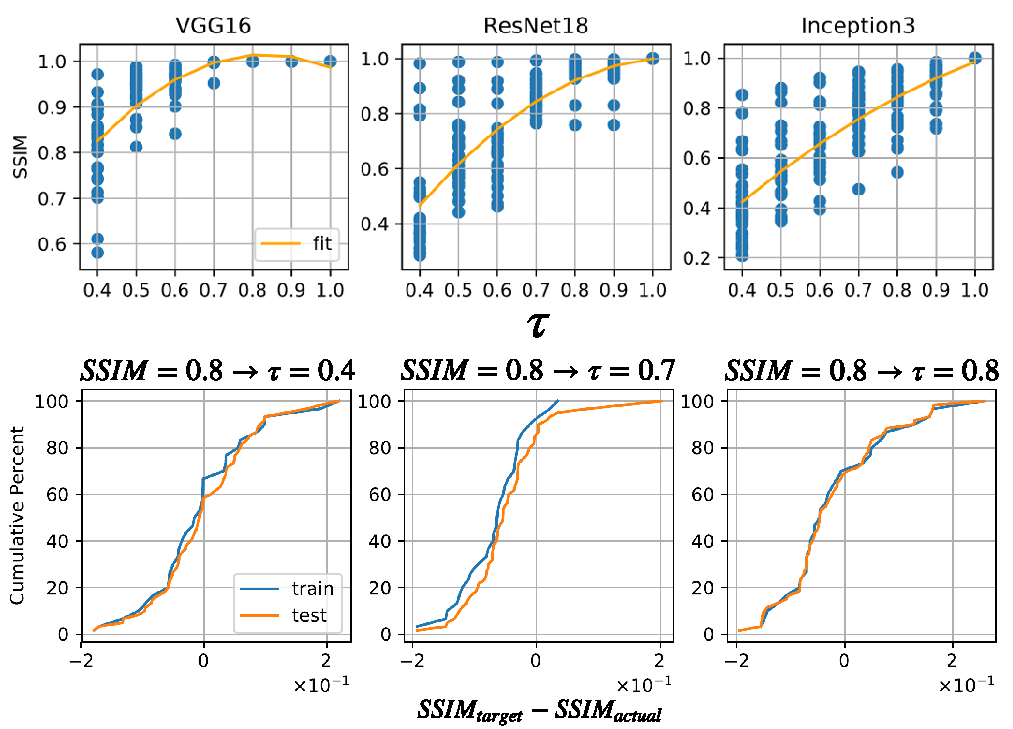
\includegraphics[width=\columnwidth]{images/system_tuning}
\caption{(a) SSIM variation and degree two curve fit for a sample of OCT dataset. (b) CDF plot for the SSIM deviation for the $\tau$ values picked from the curve fit for a target SSIM of 0.9.}
\label{fig:system_tuning}
\end{figure}

% \begin{figure}[t]
% 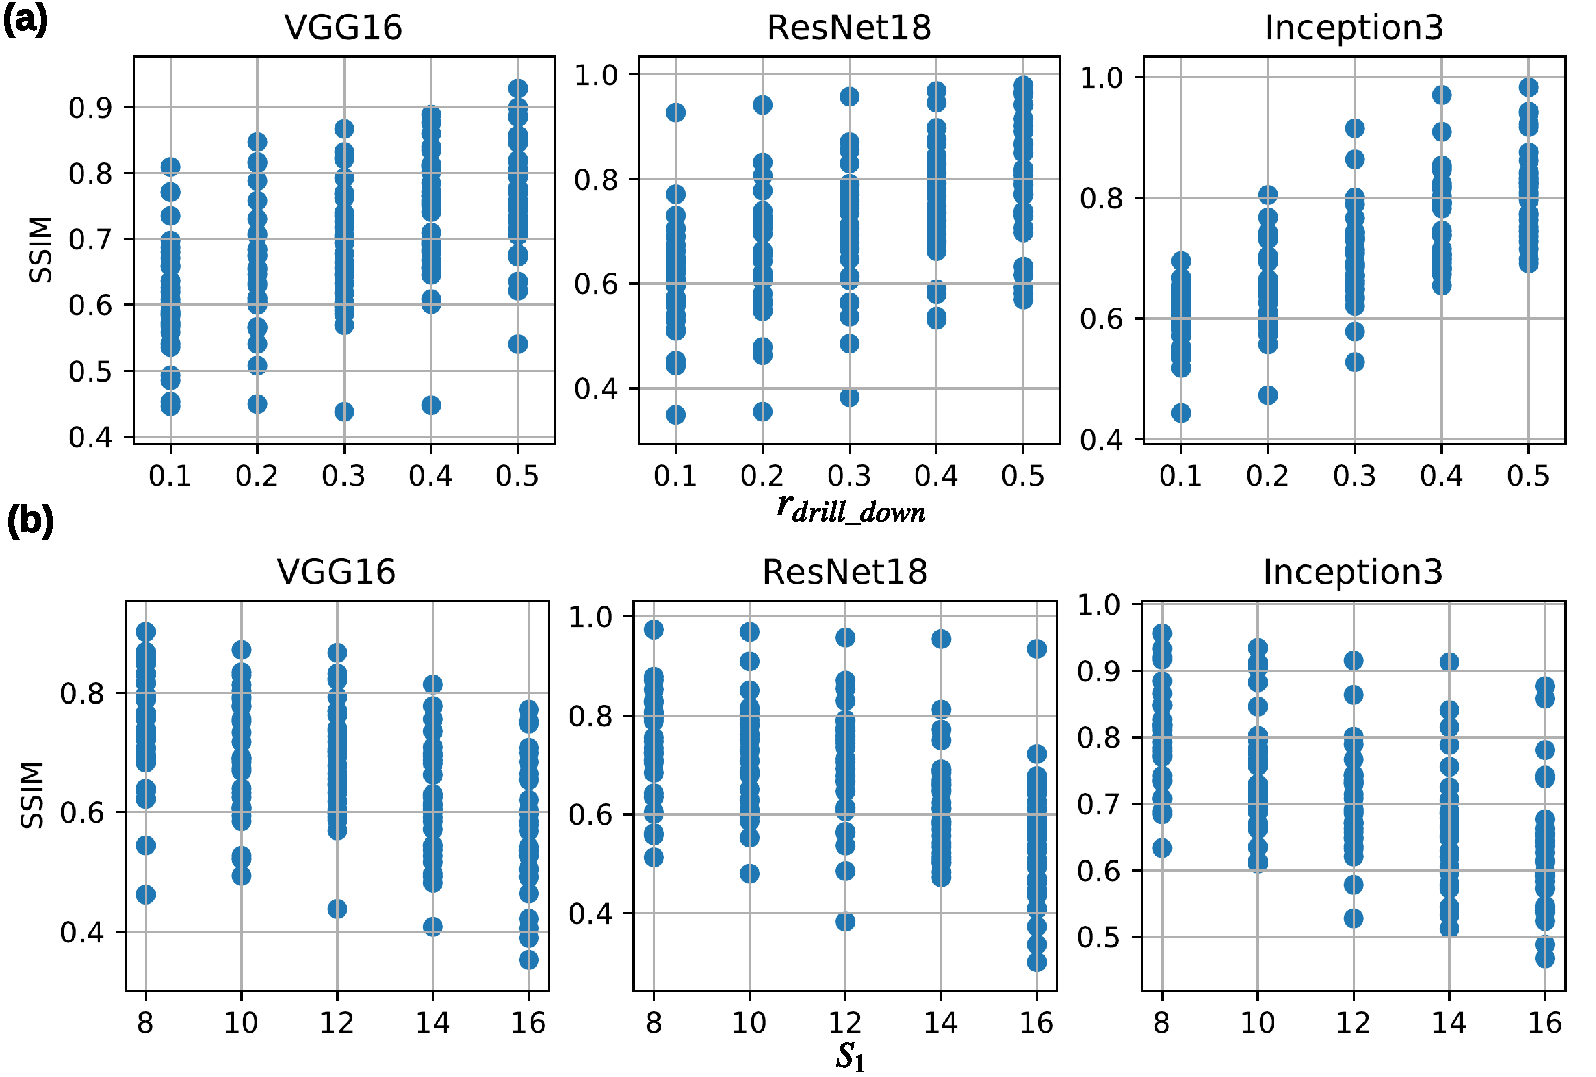
\includegraphics[width=\columnwidth]{images/adaptive_ssim}
% \caption{(a) SSIM variation for changing $r_{drill\_down}$ fixing $\tau=1$, $S_1=12$, and $S_2=4$. (b) SSIM variation for changing $S_1$ fixing $\tau=1.0$, $S_2=4$, and $r_{drill\_down}=0.3$ for a sample $(n=30)$ of OCT dataset.}
% \label{fig:adaptive_ssim}
% \end{figure}

